\chapter{State of art}\label{ch:stateofArt}
\noindent
Cooperative and non cooperative Sense and Avoid (SAA) systems are key enablers for Unmanned Aircraft (UAV) to routinely access non-segregated airspace \cite{spriesterbach2013unmanned}. Both cooperative and non-cooperative SAA systems are being developed to address this integration requirement.
\noindent
The SAA capability is defined as the automatic detection of possible conflicts by the UAV platform under consideration and performing avoidance maneuver tasks to prevent the identified collisions. An analysis of the available SAA candidate technologies and the associated sensors for both cooperative and non-cooperative SAA systems is presented in \cite{muraru2011critical}. Non-cooperative Collision Detection and Resolution (CD\&R) for UAV is considered as one of the major challenges that needs to be addressed \cite{lai2012see} for the insertion of UAVs in non-segregated air space. As a result, a number of non-cooperative sensors for the SAA system have been adopted. Light Detection and Ranging (LIDAR)is used for detecting, warning and avoiding obstacles for low-level flying \cite{sabatini2014lidar}.

An approach to the definition of encounter models and their applications to SAA strategies is presented in \cite{kochenderfer2008encounter} for both cooperative and non-cooperative scenarios.

Since 2014, there is a visible strong political support for developing rules on drones but regulations are not harmonized yet. The European Aviation Safety Agency (EASA) has been tasked to develop a regulatory framework for drone operations and proposals for the regulation of "low-risk" UAV operations. In achieving this, EASA is working closely with the Joint Authorities for Regulation of Unmanned Systes (JARUS) \cite{jarus2016regulations}.


\section{UAV motion model}
\noindent
This section strongly follows \cite{lee2011structure}.

\subsection{Continuous-time systems}\noindent
%This is very imprecise. A good notation is:
%1. u is the control function. It is a map from a time interval to \R^p, i.e., u:[0,T] \to %\R^p. Thus you could write u\in \C^p
%2. u(t) is the value (in \R^p) of the control function u. It is correct to write u(t)\in %\R^p

%You have to say what \C^p is. I guess that you mean the space of continuous functions. If this is the case, this specification is very unnatural since this space is too restrictive. Controls of interest usually have discontinuities.  More common is L^1 (space of integrable functions).

\noindent Consider a class of systems given by functions:
\begin{equation}
    \begin{split}
    S&: \vec{u}(t)  \to \vec{x}(\vec{x}_0,t) \\
    \vec{u}&(t): [0,T] \to \R^p \\
    \vec{u}&(t)\in \mathbb{R}^p , \vec{x}(t) \in \mathbb{R}^n \\
    \end{split}
\end{equation}
where $\vec{u}(t)$ and  $\vec{x}(\vec{x}_0,t)$ are a sets of continuous-time signals.
These are often called continuous-time systems because they operate on
continuous-time signals. Frequently, such systems can be defined by differential
equations that relate the input signal to the output signal.
A prototypical description of a controlled (there is a control input signal)
continuous-time system is:
\begin{equation}\label{eq:nonlinearsystem}
    \dot{x}(t) = f(t,x(t),u(t)), u(t) \in U(t)
\end{equation}
where $f:\mathbb{R}\times\mathbb{R}^n\times\mathbb{R}^p\to\mathbb{R}^n$
satisfies the conditions for existence
and uniqueness of the ordinary differential equation and $u$ is our control\cite{butcher1987numerical}.

\subsection{Discrete-time systems}
\noindent
\noindent Consider another class of systems given by functions
\begin{equation}
    \begin{split}
    S&: \vec{u}(k)  \to \vec{x}(k), \\
    k& \in \{0, t_s, 2.t_s, 3.t_s, \dots i.t_s\}, i \in \N^+\\
    \vec{u}&(k)\in \mathbb{R}^p , \vec{x}(k) \in \mathbb{R}^n\\
    \end{split}
\end{equation}
where $\vec{u}(k), \vec{x}(k)$ is a set of discrete-time signals. They can be represented by a function $f$ like $f:\{0, t_s, 2.t_s, 3.t_s, \dots i.t_s\} \to \R^n,  i \in \N^+$ where $t_s$ is sampling time and $i$ is discrete step \cite{shampine1997matlab}.

%MPC
\section{Model Predictive Control}
\noindent Model predictive control (MPC) or receding horizon control (RHC) is a form of control in which the current control action is obtained by solving on-line, at each sampling instant, a finite horizon open-loop optimal control problem, using the current state of the plant as the initial state; the optimization yields an optimal control sequence and the first control in this sequence is applied to the plant. Nearly every application imposes constraints; actuators are naturally limited in the force (or equivalent) they can apply, safety limits states such as temperature, pressure and velocity and efficiency often dictates steady-state operation close to the boundary of the set of permissible states. The prevalence of hard constraints is accompanied by a dearth of control methods for handling them, despite a continuous demand from industry that has had, in their absence, to resort often to adhoc methods. Model predictive control is one of few suitable methods, and this fact makes it an important tool for the control engineer, particularly in the process industries where plants being controlled are sufficiently slow to permit its implementation. Other examples where model predictive control may be advantageously employed include unconstrained nonlinear plants, for which on-line computation of a control law usually requires the plant dynamics to possess a special structure, and time-varying plants. 

Determining the feedback solution, on the other hand, requires solution of the Hamilton-Jacobi-Bellman differential or difference equation, a vastly more difficult task (except in those cases, such as $H_2$ and $H_\infty$.

The feedback solution provided by MPC schemes can be obtained essentially in two ways:
\begin{enumerate}
    \item \textit{Open loop control optimization} - via Maximum Principle or other techniques (e.g., approximation by linear programming).
    \item \textit{Closed loop control optimization} - via Dynamic Programming.
\end{enumerate}

\begin{figure}[H]
    \centering
    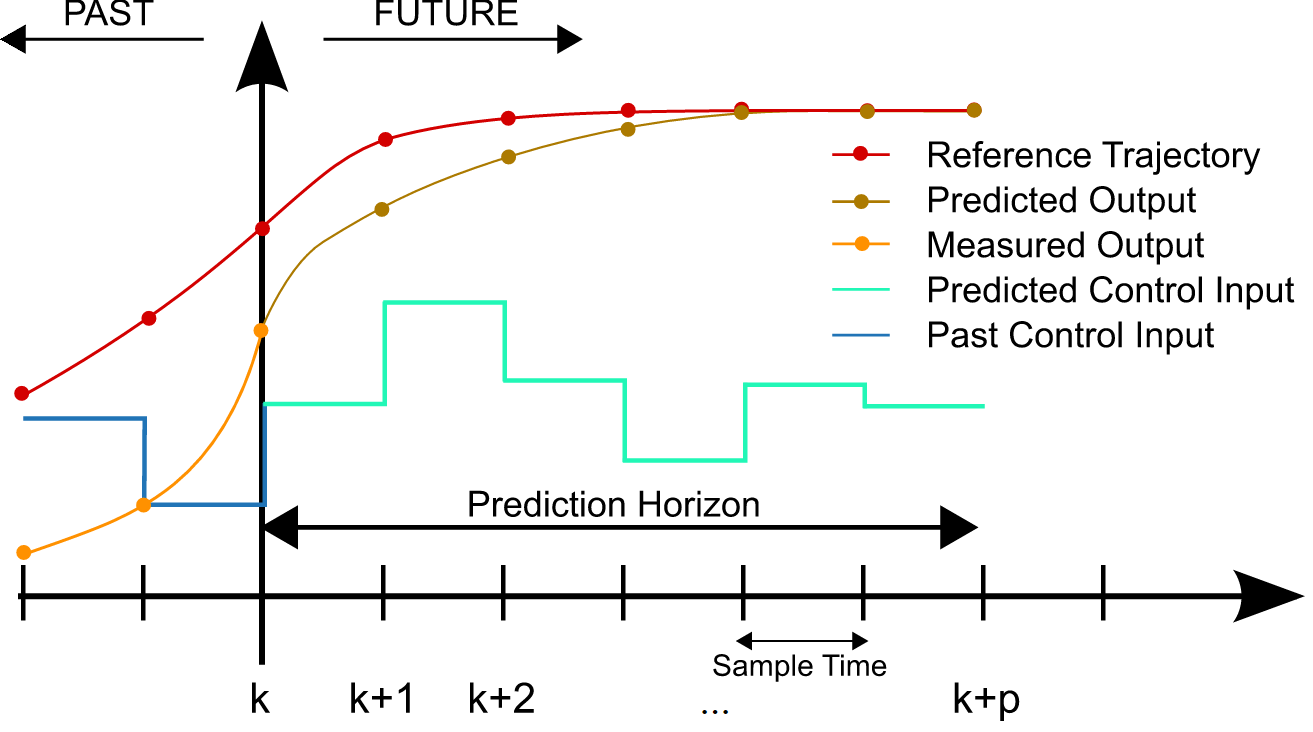
\includegraphics[width=.75\linewidth]{\FIGDIR/73_General_MPC_Scheme.png}
    \caption{General Model Predictive Control concept.}
    \label{fig:generalMPCConcept}
\end{figure}

\noindent General MPC concept is portrayed in figure \ref{fig:generalMPCConcept} for discrete time case. Usual notation is used for MPC:
\begin{enumerate}
    \item\textit{Reference trajectory} $\tilde{x}(i),i\in\left\{t_0,\dots,k,\dots,T\right\}$
    \item\textit{Predicted output} $\hat{x}(i),i\in\left\{k,\dots,T\right\}$
    \item\textit{Measured (real) output} $x(i),i\in\left\{t_0,\dots,k,\dots,T\right\}$
    \item\textit{Predicted control input} $\hat{u}(i),i\in\left\{k,\dots,T-1\right\}$
    \item\textit{Past control input} $u(i),i\in\left\{t_0,\dots,k-1\right\}$
\end{enumerate}

\noindent In general system is formulated as follow:
\begin{equation}
    \begin{aligned}
        x(k+1) &= f(x(k),u(k)), u(k)\in\mathbb{U}, x(k)\in\mathbb{X}\\
        y(k) &= h(x(k))\\
    \end{aligned}
\end{equation}
\noindent Where $f(\cdot)$ is defined by the originating differential equation that has an equilibrium point at the origin $f(\vec{0},\vec{0}) = \vec{0}$. Equation form $x^+=f(x,u)$, $y=h(x)$ is often used for shorter notation. Usually $\mathbb{U}$ is a convex compact subset of $\mathbb{R}^m$ and $\mathbb{X}$ is convex, closed subset of $\mathbb{R}^n$. For event $(x,k)$ the cost of steering is defined by function $V$:
\begin{equation}
    V(x,k,u)= \sum_{i=k}^{k+N+1}\mathpzc{l}(x(i),u(i)) + F(x(k+N))
\end{equation}
\noindent Where $u=\left\{u(k), u(k+1),\dots,u(k+N-1)\right\}$ and $x(i)= x^u(i;(x,k))$. One can assume that stage cost $\mathpzc{l}(x,u)\ge c(|(x,u)|)^2$, $\mathpzc{l}(0,0)=0$. The terminal time $k+N$ increases with time $k$ and is often referred as \textit{receding horizon}. A terminal constraint given by following equation:
\begin{equation}
    x(k+N) \in X_f \subset \mathbb{X}
\end{equation}
\noindent At event $(x,k)$ the optimal problem $\mathscr{P}(x,k)$ of minimizing cost functional $V(x,k,u)$, subject to the control, state and terminal constraint is solved yielding the optimizing control sequence:
\begin{equation}
    \hat{u}(x,k) = \left\{\hat{u}(k,(x,k)),\hat{u}(k+1,(x,k)),\dots,\hat{u}(k+N-1,(x,k))\right\}
\end{equation}
\noindent And the cost functional is equal to optimal cost:
\begin{equation}
    \hat{V}(x,k) = V(x,k,\hat{u}(x,k))
\end{equation}
\noindent The argument $(x,k)$ denotes initial state $x$ at time of prediction $k$. This defines an MPC law $\mathpzc{k}(x,k)=\hat{u}(k;(x,k))$. Since $\mathpzc{l}(\cdot)$ and $f(\cdot)$ are time invariant the problems $\mathpzc{P}(x,k)$ are invariant in the sense $\hat{V}(x,k)=\hat{V}(x,0)$ and $\mathpzc{k}(x,k)=\mathpzc{x,0}$ for all times $k$, so that is suffices, at each event $(x,k)$ to solve $\mathscr{P}_N(x,k)=\mathscr{P}(x,0)$. Problem of optimisation with finite horizon $N$ can be defined by:
\begin{equation}\label{eq:m19}
    \mathscr{P}_N(x):V_N^0(x)= \text{min}\left\{V_N(x,u)|u\in\mathscr{U}_n(x)\right\}
\end{equation}
\noindent Where $V_N(x,u)$ is given as follow:
\begin{equation}\label{eq:m110}
    V_N(x,u)= \sum_{i=0}^{N-1} \mathpzc{l}(x(i),u(i)) + F(x(N))
\end{equation}
\noindent Set of feasible control sequences $u=\left\{u(0),u(1),\dots,u(N-1)\right\}$, $x(i)=x^u(i;(x,0))$ and $\mathscr{U}_N(x)$ is the set of feasible control sequences satisfying the control, state and terminal constraints. Because the prediction horizon $N$ is finite, the minimum exists if $f(\cdot)$, $\mathbb{l}(\cdot)$ and $F(\cdot)$ are continious, $\mathbb{U}$ is compact, $X_f$ and $\mathbb{X}$ are closed. At event $(x,k)$ the problem $\mathscr{P}_N(x)$ is solved yielding the optimizing control sequence as follow:
\begin{equation}\label{eq:m111}
    \hat{u}(x)=\left\{\hat{u}(0,x),\hat{u}(1,x),\dots,\hat{u}(N-1,x)\right\}
\end{equation}
\noindent Optimal state trajectory is defined as follow:
\begin{equation}\label{eq:m112}
    \hat{x}(x)=\left\{\hat{x}(0,x),\hat{x}(1,x),\dots,\hat{x}(N,x)\right\}
\end{equation}
\noindent With value function defined as follow:
\begin{equation}\label{eq:m113}
    \hat{V}_N = V_N(x,\hat{u}(x))
\end{equation}
\noindent The single argument $\hat{x}$ denotes the initial state is $x$ at time $0$, so $\hat{x}(0,x)=x$. The first control $\hat{u}(0,x)$ is optimizing the sequence $\hat{u}(x)$ applied to the plant. The MPC law is is time invariant and is given as follow:
\begin{equation}\label{eq:m114}
    \mathpzc{k}_N(x)=\hat{u}(0,x)
\end{equation}
\noindent \textit{Dynamic programming} could in principle, be used to determine sequence $\{V_j(\cdot)\}$ of value function and a sequence of control laws $\{\mathpzc{k}_j(\cdot)\}$, where j is time to go. Because the optimal control problem is deterministic (in known environment), the value function $\hat{V}_N(\cdot)$ and its associated control law $\mathpzc{k}_N(\cdot)$ obtained via dynamic programming are \textit{identical} to the value function and control law in (\ref{eq:m113}) and (\ref{eq:m114}). It would be preferable to precompute $\mathpzc{k}_N(\cdot)$ using dynamic programming. Since this is usually impossible MPC computes at event $(x,k)$ the optimal control action $\mathpzc{k}_N(x)$ rather than pre-computing the control law $\mathpzc{k}_N(\cdot)$. The difference between MPC and Dynamic programming is in optimality guarantee. MPC with finite horizon $H_n$ gives optimal control law $\mathpzc{k}_n(\cdot)$ for given time-frame. In case that system run is longer than prediction window $n$. The control law is chained and therefore sub-optimal. Dynamic Programming guarantees optimality due it structure. Overall MPC can be seen as sequence a sequence of partial horizon optimization problems that approximates the optimization on the whole time horizon. MPC has obvious computational complexity advantages but, under favorable conditions, only guarantees a certain sub-optimality. Dynamic Programming guarantees optimality under certain conditions. Dynamic Programming usually has memory problem in long term runs.

One can find it convenient to refer to the infinite horizon value function $\hat{V}_\infty(\cdot)$ and the associated control law $\mathpzc{k}_\infty(\cdot)$ for the problem $\mathscr{P}_\infty(x)$ defined as (\ref{eq:m19}-\ref{eq:m111}), with finite horizon $N$ replaced by infinite horizon $\infty$, under assumptions that the minimum in (\ref{eq:m19}) exists.

\subsection{Stability and inverse optimality}
\noindent Model predictive control of constrained system is nonlinear necessitating the use of Lyapunov stability theory. Lyapunov stability was first proven by Chen and Shaw 1982 \cite{chen1982receding}. The value function of finite or infinite horizon can be used as Lyapunov function to establish stability of continuous time receding horizon control of unconstrained systems, when terminal equality constraint is employed. These results was extended by Mayne and Michalska \cite{mayne1990implementable} in 1990. Keerthi and Gilbert  \cite{keerthi1988optimal} first employed the value function as Lyapunov function for establishing stability of MPC of TB, constrained, non-linear discrete time systems. Therefore the value function is almost universally employed as  a natural Lyapunov function for stability analysis of model predictive control.

For any function $\Phi(x,u)$, let $\overset{\ast}{\Phi}(x,u)$ denote change in $\Phi(\cdot)$ as the state changes from $x$ to $x^+=f(x,u)$, for example $\overset{\ast}{\Phi}(x,u)=\Phi(f(x,u)-\Phi(x))$. Two distinct, but related, methods for establishing stability have evolved in the literature each yielding its own insights. Both approaches employ the value function $\hat{V}_N(\cdot)$ as a Lyapunov function. It is assumed, in the sequel that value function is continuous. The first approach, which is called \textit{direct method}, employs the value function and obtains conditions of $F(\cdot)$, $X_f$ and $\mathpzc{k}(\cdot)$ that ensures following inequality:
\begin{equation}\label{eq:m31}
    \overset{\ast}{\hat{V}}_N(x,\mathpzc{k}_N(x)) \le 0
\end{equation}
\noindent The second method uses the fact that following equality hold:
\begin{equation}
    \overset{\ast}{\hat{V}}_N(x,\mathpzc{k}(z) + \mathpzc{l}(x,\mathpzc{k}(x)))=\hat{V}_N(x^+)-\hat{V}_{N-1}(x^+)
\end{equation}
\noindent The right hand side of this equation is negative, either directly or by showing $\hat{V}_0(\cdot) \le \hat{V}_1(\cdot)$ implies $\hat{V}_{i-1}(\cdot) \le \hat{V}_i(\cdot)$, for all $i \ge 0$.

\subsection*{Direct method}
\noindent Main purpose here is to define from the expansive literature on model predictive control essential principles presented belows as axioms, that ensures closed-loop stability. This requires the determination of appropriate conditions of the ingredients $F(\cdot)$, $X_f$ and $\mathpzc{k}_f$. present in the most forms of the model predictive control. For each integer $k$, let $X_k$ denote  the set of states $x$ steerable by admissible control sequences to $X_f$ in $k$ steps or less. An admissible (or feasible) control sequence $u=\left\{u(0), u(1),\dots,u(k-1)\right\}$ satisfies the control state and terminal constraints: $u(i)\in\mathbb{U}$ for $i=0,1,\dots,k-1$, $x(i,x)\in\mathscr{X}$ for $i=0,1,\dots,k$ and $x(k,x)\in X_f$. The set of states that can be controlled by MPC with fixed horizon $N$ is $X_n$. Suppose then, that $x\in X_N$ and that the control sequence $u^0(x)$ that solves problem $\mathscr{P}_N(x)$ has been determined. Let $x^0(x)=\{x,x^0(1,x),\dots,x^0(N,x)\}$ denote the optimal state trajectory. The MPC $u=\mathpzc{k}(x)=u^0(0,x)$ steers the initial state $x$ to the successor state $x^+=x^0(1,x)=f(x,\mathpzc{k}_N(c))$. Goal is to determine a feasible control sequence $\tilde{u}(x)$ for $x^+$ to $x^0(N,x)\in X_f$. To obtain feasible control for $\mathscr{P}_N(x^+)$ one element $u$ is added to this sequence to obtain $\{u^0(1,x),\dots,u^0(N-1,x),u\}$, this sequence will be feasible for $\mathscr{P}_N(x^+)$ if $u\in\mathbb{U}$ and $u$ steers $x^0(N,x)\in X_f$ which in the case if $u=\mathpzc{k}_f(x^0(N,x))$ and $X_f$ and the local controller $\mathpzc{k}_f(\cdot)$ have following properties: $X_f \subset \mathbb{X}, \mathpzc{k}_f(x)\in\mathbb{U}$ and $f(x,\mathpzc{k}_f(x))\in X_f$, $\forall x \in X_f$ so that $X_f$ is positively invariant when the control law is $\mathpzc{k}_f(\cdot)$. If these conditions are satisfiedd the control sequence given by following equation:
\begin{equation}
    \tilde{u}(x) = \left\{u^0(1,x),\dots,u^0(N-1,x),\mathpzc{k}_f(x^0(N,x))\right\}
\end{equation}
\noindent Control sequence $\hat{u}(x)$ is feasible for $\mathscr{P}_N(x^+)$. The state trajectory resulting from initial state $x^+=x^0(1,x)$ and control sequence $\tilde{u}(x)$ is given by following equation:
\begin{equation}
    \tilde{x}(x)= \left\{x^0(1,x),\dots,x^0(N,x),f(x^0(N,x),\mathpzc{k}(x^0(N,x)))\right\}
\end{equation}
\noindent The associated cost is given by following equation:
\begin{equation}
    \begin{split}
        V_N(x^+,\tilde{u}(x)) = & V_N^0(x) - \mathpzc{l}(x,\mathpzc{k}_N(x))-F(x^0(N,x))\\
         +& \mathpzc{l}(x^0(N,x),\mathpzc{k}_f(x^0(N,x)))\\
         +& F(f(x^0(N,x),\mathpzc{k}_f(x^0(N,x))))
    \end{split}
\end{equation}
\noindent This cost which is an upper bound for $V_N^0(x^+)$ satisfies $V_N(x^+,\tilde{u}(x))\le V_N^0(x)-\mathpzc{l}(x,\mathpzc{k}_N(x))$ if $\overset{\ast}{F}(x,\mathpzc{k}_f(x))+\mathpzc{l}(x,\mathpzc{k}_f(x))\le 0$ if and only if $[\overset{\ast}{F}+\mathpzc{l}](x,\mathpzc{k}_f(x))\le 0$, $\forall x \in X_f$. Since the sum of the last three terms in the expression for $V_N(x^+\tilde{u}(x))$ is less than or equal to zero, this condition holds if $F(\cdot)$ is control Lyapunov function in the neighbourhood of the origin and $\mathpzc{k}(\cdot)$ and $X_f$ are chosen appropriately. If this condition holds, then (\ref{eq:m31}) also holds for all $x\in X_N$ which is sufficient to ensure thaht the state of closed loop system $x^+=f(x,\mathpzc{k}_N(x))$ converges to zero as $k\to\infty$ if its initial state lies in $X_N$. This motivates the following conditions that if satisfied ensure closed-loop  asymptotic stability if further minor assumptions are satisfied:

\begin{assumption}{$X_f \subset \mathbb{X}$, $X_f$ closed, $0\in X_f$ (state constraint satisfied in $X_f$)}\label{ass:m01}\end{assumption}
\begin{assumption}{$\mathpzc{k}_f(x)\in\mathbb{U}$, $\forall x \in X_f$ (control constraint satisfied in $X_f$)}\label{ass:m02}\end{assumption}
\begin{assumption}{$f(x,\mathpzc{k}(x))\in X_f$, $\forall x\in X_f$ ($X_f$ is positively invariant under $\mathpzc{k}_f(\cdot)$)}\label{ass:m03}\end{assumption}
\begin{assumption}{$[\overset{\ast}{F}+\mathpzc{l}](x,\mathpzc{k}_f(x)) \le 0$, $\forall x\in X_f$ ($F(\cdot)$ is local Lyapunov function)}\label{ass:m04}\end{assumption}

\noindent Assumption \ref{ass:m04}. implies assumption \ref{ass:m03}. if $X_f$ is a level set of $F(\cdot)$, this is a common situation. These conditions provide a concise characterization. The control sequence $\tilde{U}(x)$, in addition to providing and upper bound for $V_N^0(x)$, can also be usefully employed to initialize the algorithm for solving $\mathscr{P}_N(x^+)$. The conditions are of course merely sufficient.

\subsection*{Inverse optimality}
\noindent Bitmead et al. \cite{bitmead1990adaptive} show, in the context of linear unconstrained systems, that if the monotonicity property holds, the (finite horizon) value function $V_N^0(\cdot)$ is also the \textit{infinite horizon} value function of modified problem, an interesting example of inverse optimality. The known advantages of infinite horizon optimal control then accrue. Of course stability can be established independently as shown above. Inverse optimality can be easily extended to the nonlinear case as shown in \cite{magni1997stability}, for nonlinear unconstrained continuous time systems. The equation may be written in form:
\begin{equation}\label{eq:m33}
    V_N^0 (x) = \bar{\mathpzc{l}}(x,\mathpzc{k}_N(x))+ V_N^0(f(x,\mathpzc{k}_N(x)))
\end{equation}
\noindent For all $x\in X_N$ where $\bar{\mathpzc{l}}(x,u)=\mathpzc{l}(x,u)+[V_{N-1}^0-V_N^0](f(x,\mathpzc{k}_N(x)))$ and $\bar{\mathpzc{l}}(x,u)\ge\mathpzc{l}(x,u)\ge c|(x,u)|^2$. If assumptions \ref{ass:m01}.-\ref{ass:m04}. hold equation (\ref{eq:m33}) is fake Hamilton-Jacobi-Bellman algebraic equation corresponding to infinite horizon optimal control problem $\mathscr{P}_\infty(x)$ with $\mathpzc{l}(\cdot)$ replaced with $\bar{\mathpzc{l}}(\cdot)$. It is analogue to fake Riccati equation introduced in \cite{poubelle1988fake}. The controller $\mathpzc{k}_N(\cdot)$ is optimal for the modified problem, inherits known robustness properties of infinite horizon optimal control for nonlinear system satisfying dynamics $\dot{x}=f(x)+g(x)u$ as shown in \cite{magni1997stability}.

\subsection{Robustness}
\noindent The introduction of uncertainty in the system description raises the question of robustness, i.e. the maintenance of certain properties such as stability and performance in the presence of uncertainty. Most studies on robustness consider unconstrained systems; if a Lyapunov function for the nominal closed-loop system maintains its descent property if the disturbance (uncertainty) is sufficiently small, then stability is maintained in the presence of uncertainty. However, when constraints on states and controls are present, it is necessary to ensure, in addition, that disturbances do not cause transgression of the constraints; this adds an extra level of complexity. The earliest analyses of robustness of model predictive control employed impulse response models. Richalet study \cite{richalet1978model} investigate robustness in the face of gain mismatch. In later papers, control is determined by solving a min-max optimal control problem where the adversary represents uncertainty in the impulse response. The complexity of this problem increases exponentially with horizon length although Allwright \cite{allwright1993min} shows how this complexity may be substantially reduced. For further discussion of robustness of model predictive control using impulse response models, see \cite{zheng1993robust,genceli1993robust,de1996robustness}. It is relatively simple to ensure robust stability for linear or nonlinear systems that have finite memory finite impulse response models,finite Volterra models, etc.) since a stability constraint $x(N)=0$ is simply implementable, by choosing $N$ and $k_1$ aproppriately and imposing the constraint in the optimal control problem that the control is zero for all $k > k_1$.

There are several approaches to the study of robustness. The first is concerned with the robustness of closed-loop systems, designed using the nominal system (i.e. neglecting uncertainty). The second attempts to achieve robustness in the context of conventional model predictive control by consideration of all possible realizations on the uncertainty min-max open-loop model predictive control). A defect of model predictive control of uncertain systems, not yet widely appreciated, is the open-loop nature of the optimal control problem; the third approach addresses this by introducing feedback in the min-max optimal control problem solved on-line. 

\subsection*{Modeling uncertainty}
\noindent It should be supposed that uncertain system is  described by following equation:

\begin{equation}
    x^+ = f(x,u,w)
\end{equation}
\noindent The state $x$ and control $u$ satisfy the same constraints as before and the adversary $W$ satisfies $w(k)\in W(x(k),u(k))$ for all $k$ where, for each $(x,u)$, $W(x,u)$ is closed perhaps compact and constraints the origin in its interior. Because $f(\cdot)$ now depends on $w$ following equation is defined:
\begin{equation}
    \overset{\ast}{\Psi}(x,u,w)=\Psi(f(x,u,w))-\Psi(x)
\end{equation}
\noindent Where $\Psi(x)$ is any function. Let $w(\cdot)$ or $w=\{w(0), w(1),\dots, w(N-1)\}$ denote a disturbance sequence and $x^{u,w}(\cdot,x)$ the state trajectory resulting from an initial state $x$ at time 0, and control disturbance sequences $u$ and $w$ respectively. Let $\mathscr{F}(x,u)=f(x,u,W(x,u))$, then $\mathscr{F}(\cdot)$ maps points in $\mathbb{X}\times\mathbb{U}$ to subsets of $\mathbb{R}^n$ and $x^+\in\mathscr{F}(x,u)$ is an alternative definition of system. In some situations the uncertainty is time varying in which case uncertainty may be better modelled by $w(k)\in W_k$, where $W_k$ varies appropriately with some time $k$.

By inherent robustness is mean robustness of the closed-loop system using model predictive control obtained ignoring uncertainty. This has been investigated in \cite{de1996robustness} and \cite{magni1997stability}.

Subsequent versions of robust model predictive control that consider all realizations of the disturbance sequence $w$ in the optimal control problem require strengthened assumptions. The ingredients $F(\cdot)$, $X_f$ and $\mathpzc{k}_f(\cdot)$ are therefore assumed, to satisfy robust version of assumptions \ref{ass:m01}.-\ref{ass:m04} for stability new set of assumptions is assumed:
\begin{assumption}{$X_f\subset\mathbb{X}$, $X_f$ closed compact set, $0 \in X_f$.}\label{ass:m01a}\end{assumption}
\begin{assumption}{$\mathpzc{k}_f(x)\in\mathbb{U}$, $\forall x \in X_f$.}\label{ass:m02a}\end{assumption}
\begin{assumption} {$f(x,\mathpzc{k}_f(x),w)\in X_f$, $\forall x \in X_f $, $\forall w\in W(x,\mathpzc{k}_f(x))$}\label{ass:m03a}\end{assumption}
\begin{assumption}{$[\overset{\ast}{F}+\mathpzc{l}](x,\mathpzc{k}_f(x),w)\le 0$, $\forall x \in X_f$, $\forall w \in W(x,\mathpzc{k}_f(x),w)$. }\label{ass:m04a}\end{assumption}
\noindent There exists such a triple in $F(\cdot)$ is a robust control Lyapunov function in neighbourhood of the origin. These assumptions ensure $[\overset{\ast}{F}+\mathpzc{l}](x,\mathpzc{k}_f(x),w)\le 0$ for  all $x$ in an appropriate set and all $w\in W(x,\mathpzc{k}_N(x))$ and hence asymptotic stability.

\subsection*{Open-loop min-max model predictive control}
\noindent Deterministic model predictive control has the property that $X_N$ is positively invariant for the closed loops system $x^+=f(x,\mathpzc{k}_N(x))$. If $x\in X_N$, then $x^+ \in X_{N-1}\subset X_N$. This property is lost when uncertainty is present. To recover this property it is necessary to consider all possible realizations of $x^+ \in \mathscr{F}(x,u)$ in the optimal control problem and ensure each realization satisfies the state, control and terminal constraints \cite{michalska1993robust,chen1997game,de1999robustness}. The cost of an individual realization is defined by following equation:
\begin{equation}
    J(x,u,w) = \sum_{s=0}^{N-1} \mathpzc{l}(x(s),u(s)) + F(x(N))
\end{equation}
\noindent Where , now $x(s)=x^{u,w}(s,x,0)$ and the cost is given by following equation:
\begin{equation}
    V_N(x,u)= \text{max}\left\{J(x,u,w)|w \in \mathscr{W}_N(x,u)\right\}
\end{equation}
\noindent Where $\mathscr{W}_N(x,u)$ is the set of admissible disturbance sequences. Other choices are sometimes made for example $V(x,u)$ may be cost $J(x,u,\vec{0})$ of the nominal system, where $0$ is the zero sequence. An interesting variant, in the context of model predictive control of stable linear uncertain systems, is proposed in \cite{badgwell1997robust}; here the optimal control problem incorporates a robust stability constraint, namely that the control reduces the cost associated with each possible realization (assumed finite in number) of the linear system. This is stronger than merely a reduction in the maximum cost. In some cases ($H_\infty$ model predictive control), $\mathpzc{l}(\cdot)$ is a function of $(x,u,w)$. Let $\mathscr{U}_N^{o1}(x)$ now denote the set of admissible control sequences $u$ satisfying the state, control and terminal constraints for \textit{every} admissible  disturbance sequence $w$. when the initial state is $x$. Clearly $\mathscr{U}_N^{o1}(x)\subset\mathscr{U}_N(x)$. For all $i\ge 0$, let $X_i^{o1}$ denote the set of states $x$ such that $\mathscr{U}_N^{o1}\neq\{\}$, $X_i^{o1}\subset X_i$ is set of states that can be robustly steered to $X_f$ in $i$ steps or less by any admissible control sequence $u$. Then the optimal open-loop control problem is defined by following equation:
\begin{equation}
    \mathscr{P}_N^{o1}(x): V_N^0(x) = \text{min} \left\{V_N(x,u)|u\in \mathscr{U}_N^{o1}(x)\right\}
\end{equation}
\noindent The solution $u^0(0,x)$ of $\mathscr{P}_N^{o1}(x)$ yields the min-max MPC law given by following equation:
\begin{equation}
    \mathpzc{k}_N^{o1}=u^0(0,x)
\end{equation}
\noindent Corresponding $u^0(x)$ is a bundle of optimal state trajectories $\{X^0(x,w)\}$, one for each admissible $w$, where:
\begin{equation}
    X^0(x,w) = \left\{x^0(0,x,w),x^0(1,x,w),\dots,x^0(N-1,x,w)\right\}
\end{equation}
\noindent By the definition of $\mathscr{P}_N^{o1}$, $x^0(N,x,w)\in X_f$ for each admissible $w$. The ingredients $F(\cdot)$, $X_f$ and $\mathpzc{k}_f(\cdot)$ are assumed to satisfy assumptions \ref{ass:m01}., \ref{ass:m02}, \ref{ass:m03a}. and \ref{ass:m04a}. At this point a difficulty arises: suppose $x\in X_N^{o1}$ and optimal control sequence $\{u^0(0,x),u^0(1,x),\dots,u^0(N-1,x)\}$ steers every $x^+ \in \mathscr{P}(x,\mathpzc{k}(x))$ to $X_f$ in $N-1$ steps or less so that $x^+ \in X_{N-1}^{o1}$ The difficulty is obtaining a feasible control \textit{sequence}:
\begin{equation}
    \tilde{u}(x)=\left\{u^0(1,x),\dots,u^0(N-1,x),v\right\}
\end{equation}
\noindent For $\mathscr{P}_N(x^+)$, where $x^+$ is any state of $\mathscr{P}(x,\mathpzc{k}_N(x))$. The control action $v \in \mathbb{U}$ is required to satisfy $f(x^0(N,x,w),v\omega_N)\in X_f$ for every $w \in \mathscr{W}(x,u^0(x))$. Condition \ref{ass:m03a}. does not ensure the existence of a $v$ with this property. Without feasible sequence, an upper bound for $V_N^0(x^+)$ cannot be obtained. One way of avoiding this impasse is to replicate fixed horizon strategy by a variable horizon strategy  \cite{michalska1993robust} in which decision variable is  $(u,N)$. Suppose $u^0(x), N^0(x)$ solves the resultant variable optimal control problem $\mathscr{P}(x)$, where:
\begin{equation}
    u^0(x) = \left\{u^0(0,x), u^(1,x),\dots,u^0(N^0(x)-1,x)\right\}
\end{equation}
\noindent Then $(\bar{u}(x),N^0(x)-1)$, where:
\begin{equation}
    \bar{u}(x)=\left\{u^(1,x),\dots,u^0(N^0(x)-1,x)\right\}
\end{equation}
\noindent $\bar{u}(x)$ is a feasible solution for the optimal control problem $\mathscr{P}(x^+)$ at any $x^+ \in \mathscr{P}(x,\mathpzc{k}_N(x))$. With $V^0(\cdot)$. With $V^0(\cdot)$ denoting the resultant value function and $\mathpzc{k}^{o1}(\cdot)$ the resultant model predictive control law, where:
\begin{equation}
    [\overset{\ast}{V}^0+\mathpzc{l}](x,\mathpzc{k}^{o1}(x),w)\le 0
\end{equation}
\noindent Given monotonicity property holds for all $x \in X_N^{o1}-X_f$, all $w\in W(x,\mathpzc{k}^{o1}(x))$. Inside $X_f$, a local robustly stabilizing control law $\mathpzc{k}_f(\cdot)$. With further modest assumptions, robust asymptotic stability results with a domain of attraction $X_N^{o1}$.

\subsection{MPC for tracking}
\noindent The origin represents, with a suitable change of coordinates, any desired equilibrium state $x_r$, such that $x_r \in \mathbb{X}$, and $u_r\in\mathbb{U}$, where $u_r$ is the equilibrium control $x_r=f(x_r,u_r)$. When the system being controlled is linear, and constant input and output disturbance is present,Muske and Rawlings \cite{muske1993receding} utilize estimates of the disturbances to compute a $(x_r,u_r)$ such that the equilibrium output $x_r$ is as close as possible to the desired set-point $r$($x_r=r$ if this is possible without transgressing constraints). For further reading on tracking constant reference signals see \cite{jha2013position,lee1997stable,rawlings1994nonlinear,meadows1998feedback}. 

For tracking arbitrary reference signals (rather than those generated by a finite-dimensional exogenous system $w^+=s(w)$ variants of reference governors have been proposed. Reference governors, initially developed for control of constrained linear systems (see, for example \cite{gilbert1994nonlinear}) assume that a primal controller has been designed to stabilize the plant and provide nice tracking properties in the absence of constraints. The reference governor then modulates the $r(t)$ to obtain signal $g(t)$ with the following
properties:$g(t)$ never causes the plant to saturate and $g(t)\to r(t)$ as $t\to\infty$. Model predictive reference governors, proposed in \cite{bemporad1997nonlinear,bemporad1998fulfilling} utilize predictions over the interval reference signal $[t,t+T]$ ($t$ is currect time) to determine $g(t)$.

\subsection{Dynamic programming}\label{s:dynap}
\noindent This section adds theoretical supplements to discrete time optimisation and open possibilities of movement automaton $\mathscr{MA}$ chain optimisation. Discrete time $t_i$ is denoted as $i$, state vector $\vec{x}(t_i)$ is denoted as $x(i)$, input vector $\vec{u}(t_i)$ is denoted as $u(i)$.
\noindent Let consider problem formulation which neglects final conditions and state space constraints.
\begin{equation}\label{eq:p91}
    \begin{split}
        &\text{Maximize } \sum_{i=0}^{N-1} f_0(i,x(i),u(i)) + \Phi(x(N))\\
        &\text{Subject to: }\\
        &\textit{Dynamics: } x(i+1) = f(i,x(i),u(i)),\quad
        i = 0,1,\dots,N-1\\
        &\textit{Initial conditions: } x(0)= x_0\\
        &\textit{Control constraints: } u(i)\in\Omega_i,\quad i = 0,1,\dots
        , N-1
    \end{split}
\end{equation}
\noindent In (\ref{eq:p91}), the state $x(i)$ and the control $u(i)$ belong to arbitrary sets $X$ and $U$ respectively. $X$ and $U$ may be finite sets, or finite-dimensional vector spaces, or even infinite dimensional spaces. Initial state $x_0\in X$ is fixed. Control constraints $\Omega_i$ are fixed subsets of $U$. Finally cost function $f_0(i,\cdot,\cdot):X\times U \to \R$, $\Phi: X \to \R$, $f(i,\cdot,\cdot): X \times U \to X$ are fixed functions.


\newpage\noindent The main idea underlying \textit{dynamic programming} involves embedding the optimal control problem (\ref{eq:p91}), in which the system starts in state $x_0$ at time $0$, into a family of optimal control problems with the same dynamics, objective function, and control constraint as in (\ref{eq:p91}) but with different initial states and initial times. More precisely, for each $x \in X$ and $k$ between 0 and N - 1, consider the following
problem:
\begin{equation}\label{eq:p92}
    \begin{split}
        &\text{Maximize } \sum_{i=k}^{N-1} f_0(i,x(i),u(i)) + \Phi(x(N))\\
        &\text{Subject to: }\\
        &\textit{Dynamics: } x(i+1) =  f (i,x(i),u(i)), \quad i = k,k+1,\dots, N-1.\\
        &\textit{Initial conditions: } x(k)=x_k.\\
        &\textit{Control constraint: } u(i) \in \Omega,\quad i = k,k+1,\dots,N-1
    \end{split}
\end{equation}
\noindent Since the initial time $k$ and initial state $x$ are the only parameters in the problem above, index (\ref{eq:p92})$_{k,x}$ to distinguish between different problems.

\begin{lemma}\label{lem:p01}
Suppose $u^*(k),\dots,u^*(N-1)$ is an optimal control for (\ref{eq:p92})$_{k,x}$ and let $x^*(k) = x,x^*(k+1),\dots,x^*(N)$ be corresponding optimal trajectory $\mathscr{T}$. \\
Then for any $l,k \le l \le N-1$, control $u^*(l),\dots,u^*(N-1)$ is an optimal control for (\ref{eq:p92})$_{l,x^*(;)}$
\end{lemma}
\begin{dokaz}
Suppose that lemma \ref{lem:p01} is invalid. Then there exists control $\hat{u}(l),\hat{u}(l+1),\dots,\hat{u}(N-1)$ with corresponding trajectory $\mathscr{T} = x^*(l),\hat{x}(l+1),\dots,\hat{x}(N)$ such that:
\begin{equation}\label{eq:p93}
    \sum_{i=l}^{N-1} f_0(i,\hat{x}(i),\hat{u}(i)) + \Phi(\hat{x}(N)) > \sum_{i=l} f_0(i,x^*(i),u^x(i)) + \Phi(x^*(N))
\end{equation}
\noindent But then consider the control $\tilde{u}(k),\dots,\tilde{u}(N-1)$ given by:
\begin{equation}
    \tilde{u}(i)=
    \begin{cases}
        u^*(i), & i=k,\dots,l-1\\
        \hat{u}(i), & i=l,\dots,N-1
    \end{cases}
\end{equation}
\noindent The corresponding trajectory $\mathscr{T}$ starting at state $x$ and time $k$, is $\tilde{x}(k),\dots,\tilde{x}(N)$ is given by equation:
\begin{equation}
    \tilde{x}(i)=
    \begin{cases}
        x^*(i), & i=k,\dots,l\\
        \hat{x}(i), & i=l,\dots,N
    \end{cases}
\end{equation}
\noindent The value of the objective function corresponding to this control for the problem (\ref{eq:p92})$_{k,x}$ is given as:
\begin{equation}
    \begin{split}
        &\sum_{i=k}^{N-1} f_0(i,\tilde{x}(i),\tilde{u}(i))+ \Phi(\tilde{x}(N))\\
        & = \sum_{i=k}^{l-1} f_0(i,x^*(i),u^*(i)) + \sum_{i=l}^{N-1} f_0(i,\hat{x}(i),\hat{u}(i)) + \Phi(\hat{x}(N))\\
        & > \sum_{i=k}^{N-1} f_0(i,x^*(i),u^*(i)) + \Phi(x^*(N))
    \end{split}
\end{equation}
\noindent Equation (\ref{eq:p93}) shows that $u^*(k),\dots,u^*(N-1)$ can not be optimal for (\ref{eq:p92})$_{k,x}$, which contradicts the hypothesis. Therefore lemma is valid.
\end{dokaz}

\noindent From now on assume that an optimal solution for (\ref{eq:p92})$_{k,x}$ exists for all $0 \le k \le N-1$ and for all $x\in$. Let $V(k,x)$ be the maximum value of (9.2)$_{k,x}$. $V$ is \textit{maximum value function}.

\begin{theorem}\label{th:p01}
Define $V(N,\cdot)$ by $V(N,x)=\Phi(x)$. $V(k,x)$ satisfies backward recursion equation:
\begin{equation}\label{eq:p94}
    V(k,x) = \text{Max}\left\{f_0(k,x,u)+V(k_1,f(k,x,u))|u\in\Omega_k\right\}, 0 \le k \le N-1
\end{equation}
\end{theorem}
\begin{dokaz}
Let $x\in X$, let $u^*(k),\dots,u^*(N-1)$ be an optimal control for (\ref{eq:p92})$_{k,x}$, let $x^*(k)=x,\dots,x^*(N)$ be corresponding trajectory $\mathscr{T}^*$ and $x(k)= x,\dots,x(N)$ be another trajectory. Then following inequality holds:
\begin{equation}\label{eq:p95}
    \sum_{i=k}^{N-1} f_0(i,x^*(i),u^*(i)) + \Phi(x^*(N)) \ge \sum_{i=k}^{N-1} f_0(i, x(i), u(i)) + \Phi{x(N)}
\end{equation}
\noindent by lemma \ref{lem:p01} the left hand side of (\ref{eq:p95}) equals to:
\begin{equation}
    f_0(k,x,u^*(k)) + V(k+1,f(k,x^*,u^*(k)))
\end{equation}
\noindent On the other hand by the definition of $V$ following statement holds:
\begin{equation}
    \begin{split}
    &\sum_{i=k}^{N-1} f_0(i,x(o),u(i)) + \Phi(x(N)) =  f_0(k,x,u(k))\\
    +& \sum_{i=k+1}^{N} f_0(i,x(i),u(i)) \Phi(x(N)) \le f_0(k,x,u(k)) + V(k+1,f(k,x,u(k)))
    \end{split}
\end{equation}
\noindent With equality if and only if $u(k+1),\dots,u(N-1)$ is optimal for (\ref{eq:p92})$_{k+1,x(k+1)}$. Combining these two factors we get following inequality:
\begin{equation}
    \begin{split}
    &f_0(k,x,u^*(k)) + V(k+1,f(k,x,u^*(k)))\\
    \ge & f_0(k,x,u(k)) + V(k+1,f(k,x,u(k)))
    \end{split}
\end{equation}
\noindent for all $u(k)\in\Omega_k$ which is equivalent to equation (\ref{eq:p94}) form theorem.
\end{dokaz}

\begin{corollary}
Let  $u(k),\dots,u(N-1)$ be any control for problem (\ref{eq:p92})$_{k,x}$ and let $x(k) = x,\dots,x(N)$ be the corresponding trajectory. Then following equality holds tor all $k \le l \le N-1$  if and only if the control is optimal for (\ref{eq:p92})$_{k,x}$:
\begin{equation}
    V(l,x(l)) \le f_0(l,x(l),u(l)) + V(l+1,f(l,x(l),u(l))), \forall l, k \le l \le N-1
\end{equation}
\end{corollary}
\begin{corollary}
For $k=0,1,\dots,N-1$, let $\psi(k,\cdot): X\to \Omega_k$ be such that:
\begin{equation}
    \begin{split}
    & f_0(k,x,\psi(k,x))+ V(k+1,f(k,x,\psi(k,x)))\\
    =&\text{Max}\left\{f_0(k,x,u)+ V(k+1,f(k,x_u))|u\in\Omega_k\right\}
    \end{split}
\end{equation}
\noindent Then $\psi(k,\cdot), k = 0,\dots,N-1$ is an \textit{optimal feedback control}, therefore for any $k,x$ the control $u^*(k),\dots,u^*(N-1)$ defined by $u^*(l)=\psi(l,x^*,(l)), k \le l \le N-1$ is optimal for (\ref{eq:p92})$_{k,x}$: if following equation holds:
\begin{equation}\label{eq:pcol2}
    x^*(l+1)=f(l,x^*(l),\psi(l,x^*(l))), k \le l \le N-1, x^*(k)=x
\end{equation}
\end{corollary}
\noindent Theorem \ref{th:p01} and corollary (\ref{eq:pcol2}) are the main results of dynamic programming. The recursion equation (\ref{eq:p94}) allows to compute the value function and in evaluating the maximum in (\ref{eq:p94}) one can also obtain the optimum feedback control. Note that this feedback control $\psi$ is optimum for all initial conditions, However unless we can find a \textit{closed form} analytic solution to (\ref{eq:p94}), the dynamic programming formulation may necessitate a prohibitive amount of computation, since we would have to compute and store the values of $V$ and $\psi$ for all $k$ and $x$.

The most common application of \textit{Dynamic Programming} is application to problems in operation research where one can obtain “closed-form” analytic solutions to be recursion equation for the \textit{value function} \cite{re1962applied,wagner1969principles}. In the case of \textit{sequential decision-making under uncertainties}, where \textit{Sense\&Avoid} in full form belong, \textit{Dynamic Programming} is about the only available general method \cite{howard1960dynamic}. Larson \cite{larson1968state} has developed computational techniques which greatly increase the range of applicability of \textit{Dynamic Programming} where closed-form solutions are not available. These results can be reused in case of movement automaton $\mathscr{MA}$.
% REACH SETS
\section{Reach sets}

\subsection*{Definition}
\noindent
The reach set of a system described by a differential equation is the
set of all states that can be reached from an initial state within a given time
interval.
\noindent For general case consider the system described by equation (\ref{eq:nonlinearsystem}).

\begin{definition}[Reach set starting at a given point]\label{def:reachset01}
Suppose the initial position
and time $(\vec{x}_0, t_0)$ are given. The reach set $\mathscr{R}[\tau; t_0, \vec{x}_0]$ of system (\ref{eq:nonlinearsystem}) at time $\tau \ge t_0$, starting at position and time $(\vec{x}_0, t_0)$ is given by:
\begin{equation}
    \mathscr{R}[\tau, t_0, \vec{x}_0] = \bigcup \{\vec{x}(\tau):\vec{u}(s)\in U(s),s \in (t_0,\tau]\}
\end{equation}
\end{definition}
\noindent Reach set starting at given set can be used to determine reach set in case of hybrid system input control switch and it is defined as follow:
\begin{definition}[Reach set starting at a given set]
The reach set at time $\tau > t_0$ starting from set $X_0$ is defined as:
\begin{equation}
    \mathscr{R}[\tau, t_0, X_0] = \bigcup \{R[\tau, t_0, \vec{x}_0]:\vec{x}_0 \in X_0\}
\end{equation}
\end{definition}

\newpage\noindent Reach set for adversarial behavior can be used to calculate possible escape routes from pursuer and it is defined as follow:
\begin{definition}[Reach set under adversarial behavior]
Consider now the case of adversarial behavior, for system $\dot{x}=u,u\in \mathbb{B}$.
where $u(t)$ is our control and $v(t)$ is adversary control which is independent of $u(t)$, let $w(t)=u(t)- \arg_{v(t)\in V(t)}\sup_{{x} \in x(t)} v(t)$, which represents worst possible input change in given state and time, then reach set for system is represented as:
\begin{equation}
    \mathscr{R}[\tau; t_0, \vec{x}_0] = \bigcup \{\vec{x}(\tau):\vec{w}(s) \in W(s),s \in (t_0,\tau]\}
\end{equation}

\end{definition}

\noindent Reach set under constraints are usable to define state constrained systems in terms of dynamics and technical capabilities.
\begin{definition}[Reach set under state constraints]
Suppose the initial position
and time $(\vec{x}_0, t_0)$ and $x$ constraints are given $x(t) \in \mathbb{A} \subset \R^n, \dot{x}(t) \in \mathbb{B} \subset \R^n$. The reach set $\mathscr{R}[\tau, t_0, \vec{x}_0]$ of system (\ref{eq:nonlinearsystem}) at time $\tau \ge t_0$, starting at position and time $(\vec{x}_0, t_0)$ is given by:
\begin{equation}
    \mathscr{R}[\tau, t_0, \vec{x}_0] = \bigcup \{\vec{x}(\tau):\forall s\in (t_0,\tau], x(s) \in \mathbb{A}, \dot{x}(s) \in \mathbb{B}, \exists u(s) \in U(s)\}
\end{equation}
\end{definition}

\section{Occupied space}
\noindent Occupied pace representation is crucial in obstacle avoidance, this section introduces models and notations. Analytical geometry structures of sphere and ellipsoid are used to  determine closed occupied spaces.
\begin{definition}{Unit sphere (Unit ball) $\mathscr{B}(\vec{p},r)$} denotes occupied space in point $\vec{p} = [x_p,y_p,z_p]^T$ with radius $r$. Where point $\vec{b} = [x_b,y_b,z_b]$ belongs to sphere $\mathscr{B}(\vec{p},r)$ if and only if:
\begin{equation}
    (x_b-x_p)^2 + (y_b-y_p)^2 + (z_b-z_p)^2 \le r
\end{equation}    
\end{definition}
Definition of sphere $\mathscr{B}(\vec{p},r)$ is usually used to denote safety margin of vehicle $s_m$, where $s_m$ represents maximum radius to vehicle matter point from vehicle mass center. 
\begin{definition}{Spherical coating $\mathscr{C}(\vec{f}(\cdot),r)$} denotes occupied space of object which surface can be approximated by function $f(\cdot)$, with points of surface $\vec{p}=[x_p,y_p,z_p]^T\in\R^3$ and object inner points $\vec{i}=[x_i,y_i,i_p]^T\in \R^3$. Then spherical coating $\mathscr{C}(\vec{f}(\cdot),r)$ is defined as follows:
\begin{equation}
    \mathscr{C}(\vec{f}(\cdot),r) = \left\{\vec{b} \in \R^3: \vec{b}\in \bigcup_{\forall \vec{p} \in \vec{f}(\cdot)} \mathscr{B}(\vec{p},r), \nexists \vec{i}=\vec{b}  \right\}
\end{equation}
One can say that spherical coating is a closed,not compact set of points $\vec{b} = [x_b,y_b,z_b]$  where distance to closest surface point $\vec{p}$ is lesser or equal to coating radius $r$.    
\end{definition}
\noindent Calculation of spherical coating can be time consuming especially when surface function $\vec{f}(\cdot)$ is not smooth \cite{sommerville2016analytical}. Closest point problem has been formulated by Shamos \cite{shamos1975closest}.Closest point estimation with moving vehicle and with thick data flow can by solved by time optimal and deterministic approach, one of them have been presented by Bentley in \cite{bentley1980optimal}. Approach is based on closest point search in local planar coordinates which may be ideal for steam-line LiDAR data. 
Estimation of spherical coating is used in potential field avoidance methods. One most notable study was using spherical approximation based on obstacle center and mass distribution in space \cite{borenstein1991vector}. Potential field have their limitations in partially known environment, because it is hard to determine center of mass and mass distribution of obstacle from partial information \cite{koren1991potential}. Main source of object proportional estimation can be reused from camera based solutions like \cite{oberkampf1993iterative}. Other possible solution sources from fast clustering algorithms from Geographical Information Systems (GIS) for example \cite{zaiane2002clustering}.

\section{Movement automaton}
\noindent Movement automaton used as proxy between discrete command chain (movement chain) and control signal ($u(t)$). Movement automation is based on hybrid automaton.
\begin{definition} {Hybrid automaton $\mathscr{H}(Q,\R^n,f,\varphi,\rho)$} is well defined system representation consisting from following components.
\begin{equation}
    \begin{aligned}
        Q &\equiv \textnormal{set of discrete states}\\
        \R^n &\equiv \textnormal{continuous state-space} \\
        f: Q\times \R^n \to \R^n & \equiv \textnormal{vector field}\\
        \varphi:Q\times \R^n \to Q & \equiv \textit{discrete transition}\\
        \rho : Q\times \R^n \to \R^n & \equiv\textit{reset map}\\
    \end{aligned}
\end{equation}
Discrete state $q_i \in Q$ represents system current state and impacts system behavioural equation and state. Continuous state $[x(t),u(t)]\in \R^n$ represents  system state from physical viewpoint (values of state variables and inputs in continuous space $\R^n$). Vector field $f$ assign to each discrete state $q_i \in Q$ system behavioral function $\dot{x} = f(x,u)$. Discrete transition $\varphi$ defines conditions to transit between two different states. Reset map $\rho$ defines system state or input change on reset conditions.
\end{definition} 

\begin{definition}{Trajectory primitive $\hat{t}(x_0,t_0,t_1)$} is defined on given time interval $(t_0,t_1]$ for system $\dot{x} = f(x,u)$ with initial state $x_0$ at $t_0$ and final state $x_1$ at $t_1$ as follow:
\begin{equation}
    \hat{t}(x_0,t_1,t_1) = \left\{ x\in\R^n: x = \Phi(t_0,\tau,x_0), \tau \in (t_0,t_1] \right\}
\end{equation}
Trajectory primitive can be viewed as ordered set of system trajectory positions, this set is infinite continuous and flat.    
\end{definition}

\begin{definition}{Trajectory equivalence.}
Let $\mathscr{T}$ be trajectory defined as ordered sequence of countable trajectory primitives:
\begin{equation}
    \mathscr{T} = \left\{ \bigcup_{i=0}^n \hat{t}_i(x_i,t_i,t_{i+1}) \right\}
\end{equation}
Trajectory $\mathscr{T}$ is time independent and contains at leas one trajectory primitive. Trajectory $\mathscr{T}_\alpha$ consist from $m\ge 1$ trajectory primitives and its smooth and continuous. Trajectory $\mathscr{T}_\beta$ consist from $n \ne m$ primitives and its smooth and continuous.  Trajectories $\mathscr{T}_\alpha \equiv \mathscr{T}_\beta$ if and only if:
\begin{equation}
    \forall x_i \in \mathscr{T}_\alpha \exists y_i \in \mathscr{T}_\beta: x_{i+1} \equiv y_{i+1}, i \in {0\dots k}
\end{equation}
Where $x_i$ and $y_i$ is i-th point of trajectorries in state space $\R^n$.
\end{definition}

\noindent Trajectory primitives and trajectory equivalence have been defined, therefore movement primitives and movement can be defined.

\begin{definition}{Movement primitive $p$} 
for system $\dot{x} = f(x,u)$ and time interval $(t_i,t_{i+1}]$ there is defined continuous input signal $u(t)$.
\begin{equation}
    p_i = u(t), t\in (t_i,t_{i+1}]
\end{equation}
\end{definition}

\noindent Movement primitives can be chained to give smooth input signal. if there is movement primitive $p_1$ and movement primitive $p_2$ they can be chained on time $\tau$ when $u_1(\tau) = u_2(\tau)$, therefore system state can be also chained $x_1(\tau) = x_2(\tau)$.
\begin{definition}{Movement m(t)} is defined as chain of movement primitives $\{p_1,p_2,\dots,p_n\}$. Movement is smooth function with existing derivation. 
\end{definition}
\noindent Movement is main building block of movement automaton, movement is defined by movement type and its duration, movement switching is possible when execution time allows movement chaining. Movements can be separated into two categories:
\begin{enumerate}
    \item \textit{Stationary movement} - movement signal is constant during time of movement execution
    \item \textit{Dynamic movement} - movement signal is evolving during time of movement execution.
\end{enumerate}
\begin{definition} {Movement automaton $\mathscr{MA}$}\label{def:movementAutomaton} for system defined by dynamics $\dot{x} = f(x,u)$ is a structure defined as follow:
\begin{equation}
    \begin{aligned}
    M&\equiv\textnormal{set of movements}\\
    u:M\times\R\to\R^m&\equiv\textnormal{input function evolution}\\
    \varphi:M\times M \times \R&\equiv\textnormal{movement transition map}\\
    B=M\times\R^2&\equiv\textnormal{movement buffer}\\
    \end{aligned}
\end{equation}
Movement $m_i\in M$ can be stationary or dynamic. Each movement in movement buffer has assigned duration $(t_i,t_{i+1}]\in\R^2$. Input function evolution $u(B,t)$ defines input evolution in given execution time $t = \tau+t_0, \tau\in(t_0,t_1]$.
Each movement $m_i$ in movement automaton $\mathscr{MA}$  is compliant with following rules:
\begin{enumerate}
    \item Each movement $m_i(t_{i},t_{i+1})$ has non zero duration.
    \item At switching time $\tau$ between movements $m_i$ and $m_{i+1}$, input function $u_i(\tau + t_i) = u_{i+1}(0)$.
    \item Each dynamic movement should be linking two static movement and vice-versa.
\end{enumerate}
\end{definition}

\newpage\subsection{Prediction stability of Movement Automaton}\label{s:maConvergence}
\noindent Because Movement automaton $\mathscr{MA}$ is abstract level control realized trough \textit{open loop hybrid automaton}, infinite receding horizon is questionable. This fact impacts the prediction reliability. This subsection formulates \textit{prediction horizon of movement automaton}.

\begin{definition}{Movement automaton $\mathscr{MA}$ prediction stability}\label{def:maPredictionStability}
For system $\dot{x}=f(x,\mathscr{MA})$ and predictor $\dot{\hat{x}}=f(\hat{x},\mathscr{MA})$ with separable nonlinear state $h(\cdot)$ and input transformation $g(\cdot)$ functions. With initial condition $x(t_0)=\hat{x}(t_0)=x_0$ and finite execution time $t\in[t_0,t_1]$. Prediction deviation $x(t)-hat(x)(t)$ stays in unit ball defined by:
\begin{equation}
    \mathscr{B}(x(t)-\hat{x}(t))= \left\{y\in\R^n:y=x(t)-\hat{x}(t),\norm{y}\le\rho\right\}
\end{equation}
\end{definition}

\begin{dokaz}
Let $\dot{x}=f(x,\mathscr{MA})$ be continuous time system, with state $x\R^n$ and control with movement automaton $\mathscr{MA}$. Input function $u(t)$ for movement buffer $B=\{m_1(t_1),\dots,m_i(t_i)\}$ is interpreted as chained input function:
\begin{equation}\label{eq:maTranslation}
    u(t)=
    \begin{cases}
        u(m_0,m_1,t_0,t_1)&:\textnormal{for } m_1(t_1)\\
        \vdots&\\
        u(m_{i-1},m_{i},t_{i-1},t_{i})&:\textnormal{for } m_i(t_i)
    \end{cases}
\end{equation}
\noindent Input function $u(t)$ (\ref{eq:maTranslation}) is smooth and differentiable as given by movement automaton $\mathscr{MA}$  definition (def. \ref{def:movementAutomaton}.). Let $w(t)$ be state noise function with boundary $\xi_w\in\R-\{\infty\}$, $v(t)$ input noise function with boundary $\xi_v\in\R-\{\infty\}$ and $\hat{x}(t)$ predicted state for movement chain $B=\{m_1(t_1),\dots,m_i(t_i)\}$. We can define function $V(t)$ as follow:
\begin{equation}
    V(t) = \frac{1}{2} (x(t)-\hat(x){t})^T\text{I}(x(t)-\hat(x)(t)) = (x(t)-\hat{x}(t))^2
\end{equation}
\noindent Given function can be derived by time $t$: 
\begin{equation}
    \dot{V}(t) = x(t)-\hat(x)(t)
\end{equation}
\noindent Controlled system with state $w(t)$ and input noise $v(t)$, where input and state are separable:
\begin{equation}
    \dot{x}=f(x,\mathscr{MA}) = g(x(t)+ w(t)) + h(u(t)+ v(t))
\end{equation}
\noindent Predicted system equation:
\begin{equation}
    \dot{\hat{x}}=f(\hat{x},\mathscr{MA}) = g(\hat{x}(t)) + h(u(t))    
\end{equation}
\noindent Therefore $\dot{V}$ is equal to:
\begin{equation}
    \begin{split}  
    \dot{V}(t) &= (g(x(t)+ w(t)) + h(u(t)+ v(t))) - (g(\hat{x}(t)) + h(u(t)))\\
               &=  g(w(t)) + h(v(t))
    \end{split}
\end{equation}
\noindent Member $g(x(t)-\hat{x}(t))$ is equal to zero, because of the premise that predicted $\hat{x}$ and real state $x$ are equal without state $w(t)$ and input noise $v(t)$ noise. Let us bound $g(w(t))$, boundary is straightforward in this case, because state noise $w(t)$ is bounded by $\xi_w$. Boundary is given as:
\begin{equation}
    \norm{g(w(t))} \le \norm{g(_{sup}(w(t)))} \le \norm{g(\xi_w)} \le \rho_w,\quad \rho_w\in\R^+-\{\infty\}
\end{equation}
\noindent Bounding member $h(v(t))$ will be problematic due to mapping function (\ref{eq:maTranslation}). Introducing input noise to movement automaton mapping function will cause input noise to be characterized like this:
\begin{equation}
    u(t)-\hat{u}(t)=\left(
    \begin{cases}
        u(m_0,m_1,t_0,t_1)+v_1(t)&\\
        \vdots&\\
        u(m_{i-1},m_{i},t_{i-1},t_{i})+v_i(t)^i&
    \end{cases}
    \right) -\left(
    \begin{cases}
        \hat{u}(m_0,m_1,t_0,t_1)&\\
        \vdots&\\
        \hat{u}(m_{i-1},m_{i},t_{i-1},t_{i})&
    \end{cases}
    \right) 
\end{equation}
\noindent This can be simplified to:
\begin{equation}
    \sum_{l=0}^{i} v_l(t)^l, \quad i\in\R^{+}-\{0,\infty\}
\end{equation}
\noindent So for case of input noise $v(t)$ member $h(v(t))$ of $\dot{V}(t)$ can be bounded like follow:
\begin{equation}
    \norm{h(v(t))} \le \norm{h(_{sup}\sum_{l=0}^{i} v_l(t)^l)}\le \norm{h(\xi^i)} \le \rho_v \quad \rho_v\in\R^+-\{\infty\}
\end{equation}
\noindent Where $i$ is finite count of movements in movement automaton $\mathscr{MA}$ buffer $B$, $i=|B|$. This parameter is cumulative which is given by member $\norm{h(_{sup}\sum_{l=0}^{i} v_l(t)^l)}$, but it is bounded by $\norm{h(\xi^i)}$. One can define boundary as follow:
\begin{equation}
    \norm{\dot{V}(t)} \le \rho_w + \rho_v = \rho, \quad \rho\in\R^+-\{\infty\}
\end{equation}
\noindent With boundary defined for derivation of $V(t)$ one can define boundary for $V(t)$ like follow for time of prediction $t_0$ and time of movement buffer execution end $t_i$:
\begin{equation}
    \norm{V(t)} \le \int_{t_0}^{t_i} \norm{\dot{V}(t)}\quad \text{d}t \le \int_{t_0}^{t_i} \rho \quad\text{d}t = \rho(t_i-t_0)
\end{equation}
\end{dokaz}
\subsection{Lyapunov stability of Movement Automaton}\label{s:maLyapunov}
\noindent It has been proven that system with movement automaton is stable in terms of finite receding horizon prediction. There is still open issue of \textit{Lyapunov stability}. To prove Lyapunov stability one needs to construct tracking problem of waypoint. Let say that system initial state $x(t_0)\in \mathscr{B}_s \subset \R^n$ is unit ball where system $\dot{x} = g(x) + h(u)$ is trying to reach equilibrium point $\hat{x}(t_i)$. Equilibrium point is predicted state $\hat{x}$ at final time of movement automaton $\mathscr{MA}$ buffer execution $t_i$. Then region of attraction $\mathscr{B}(\hat{x}(t_i),\rho)$, where $\hat{x}(t_i)$ is center of unit ball and $\rho$ is prediction deviation boundary at time $t_i$ given by definition (def. \ref{def:maPredictionStability}). Let us define system $y$ for tracking problem with equilibrium point $x(t_i)$ and initial state $x(t_0)\in\mathscr{B}_s$ for finite time period $t_\in[t_0,t_i]$
\begin{equation}
    y = {x}(t)-\hat{x}(t_i), \quad x(t_0)\in\mathscr{B}_s\subset\R^n, 
\end{equation}
\noindent It is obvious that region of attraction $\mathscr{B}(\hat{x}(t_i),\rho)$, is subset of $\mathscr{B}_s$. Let us define simple Lyapunov function $V(y)$ like follow:
\begin{equation}
    V(y) = \frac{1}{2}y^Ty = \frac{1}{2}\sum_{l=1}^n\left(x_l(t)^2-\hat{x}_l(t_i)^2\right)
\end{equation}
\noindent With derivation in time given by equation:
\begin{equation}
    \dot{V}(y)= \sum_{l=1}^n \frac{\partial V(y)}{\partial y_l}
\end{equation}
\noindent Now lets check second Lyapunov method stability conditions for $y$:
\begin{enumerate}
    \item $V(0)=0$ - this condition is valid, because Lyapunov function is 0 at equilibrium point $\hat{x}(t_i)$.
    \item $V(y) < 0, \forall y\in\mathscr{B}_s-\{0\}$ - this condition is valid, because $\frac{1}{2}\norm{y}>0,\forall y\in\mathscr{B}_s-\{0\}$.
    \item $\dot{V}(y)<0$ or $\dot{V}(y)\le0$ - convergence criterion is fully satisfied in case of no existing obstacle, because avoidance framework converges to goal waypoint exponentially fast.
\end{enumerate}
\noindent Convergence condition $\dot{V}(y)<0$ is not guaranteed in term of obstacle avoidance, because in some cases $\dot{V}(y)>0$ while avoiding enormous obstacle. Movement automaton $\mathscr{MA}$ is exponentially or at least asymptotic stable in terms of Lyapunov stability, within region of attraction $\mathscr{B}(\hat{x}(t_i),\rho)$. Obstacle avoidance framework is can be or can not be Lyapunov stable depending on obstacle set $\mathscr{O}$. Reachibility of waypoint $\hat{x}(t_i)$ is determined by system reachibility set $\mathscr{R}$.

\section{LiDAR}
\noindent LiDAR (Light Detection And Ranging) is active form of remote sensing: information is obtained from a signal which is sent from a transmitter and reflected by a target, and detected by a receiver back at the source. Following types of information can be obtained:
\begin{enumerate}
\item \textit{Range to target} - topographic LiDAR or laser altimeter.
\item \textit{Chemical properties of target} - differential absorption LiDAR.
\item \textit{Velocity of target} - Doppler LiDAR.
\end{enumerate}

\noindent Chemical properties of target are out of scope. Velocity of  target seems as interesting property to investigate, but this type of LiDAR is usually used for meteorological measurements of wind currents \cite{martin2011meteorological}. Extended research in LiDAR as obstacle detection sensor has been executed by research group around Sabatini \cite{sabatini2014lidar} and Ramasy \cite{ramasamy2016lidar}. 

LiDAR output is represented as point cloud it is described by following definition.
\newpage\begin{definition}[Scanned point and Point-cloud]
Consider viewpoint $v$ as origin of $\R^3$ space in 
Let point $p \in P$ be defined in polar coordinates:
\begin{equation}
    p= [ d, \theta, \varphi, t ]^T
\end{equation}
Where $d$ is distance to scanner, $\theta$ is horizontal angle from origin, $\varphi$ is vertical angle to origin, $t$ is time of retrieval.\\

\noindent Point-cloud is set of points scanned in small enough time-frame, based on processing raw point data it can have following representations:
\begin{enumerate}
\item Local point-cloud - position of sensor is used as origin of space and points can be represented in orthogonal or planar representation. 
\item Global point-cloud -global position of sensor is used as reference to calculate global position of points.
\end{enumerate}
\end{definition}

Point-cloud is usually addressed as \textit{raw point-cloud} in case if its represented in Local planar coordinates. Other forms of point cloud require further processing and they are not feasible for real time obstacle detection and avoidance \cite{chen2007airborne}.

\begin{figure}[H]
    \begin{subfigure}{0.5\textwidth}
    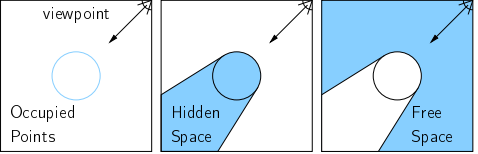
\includegraphics[width=0.9\linewidth]{\FIGDIR/10_Lidar_sets1.PNG} 
    \caption{Space type definitions}
    \label{fig:Spacetypes}
    \end{subfigure}
    \begin{subfigure}{0.5\textwidth}
    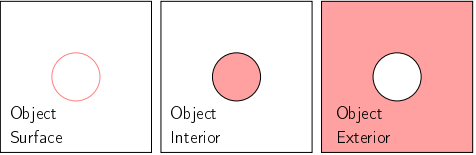
\includegraphics[width=0.9\linewidth]{\FIGDIR/11_Lidar_sets2.PNG}
    \caption{Object properties definitions}
    \label{fig:ObectProperties}
    \end{subfigure}
    \caption{Six spaces of interest \cite{yapo2008probabilistic}}
    \label{fig:Spaces of interests}
 \end{figure}
 
\noindent  Because of real-time obstacle avoidance it is necessary to introduce following terminology:
 \begin{enumerate}
 \item \textit{Occupied points} - points which have been detected by LiDAR (also addressed as visible points).
 \item \textit{Hidden space} - space which is hidden behind occupied points, from viewpoint it is uncertain what is in that space. 
 \item \textit{Free space} - space which is visible from viewpoint and it is not occupied by known objects.
 \item \textit{Object surface} - detected and undetected object surface
 \item \textit{Object interior} - occupied space by object.
 \item \textit{Object exterior} - free space around known objects.
 \end{enumerate}
 Existing method for space segregation \cite{yapo2008probabilistic} can yeld to following definition.
 \begin{definition}[Accessible space]\label{def:accessibleSpace}
    Consider known space $S$ as space explored by sensor (it can have different viewpoint along previous 3D trajectory).
    Intersection between \textit{object exterior} $S_E$ and \textit{free space}$S_F$ gives us \textit{Accessible space}.
    \begin{equation}
        S_A = S_E \cap S_F
    \end{equation}
 \end{definition}
 
 \noindent Accessible space $S_A$ (\ref{def:accessibleSpace}) is our bordering limitation for reachable space of system $R(\tau,t_0,\vec{x_0})$ (def. \ref{def:reachset01}.); 